% ==============================================================================
% SEÇÃO 13: TELAS DO FRONT-END E FLUXOS ASSISTENCIAIS (ITEM 13)
% ==============================================================================

\section{Telas do Front-End e Fluxos Assistenciais da Aplicação (Item 13)}
\label{sec:telas_frontend}

Esta seção apresenta as capturas de tela reais da interface web do Sistema Vitalis (construída em \textbf{React~19}, \textbf{TypeScript}, \textbf{Vite}, \textbf{Tailwind CSS} e \textbf{TanStack Query}), extraídas por automação \textit{Playwright} diretamente da aplicação em operação integrada aos quatro serviços de back-end e ao provedor local de inteligência artificial (\textit{Ollama} com o modelo \texttt{qwen2.5:7b-instruct-q5\_K\_M}).

% ==============================================================================
\subsection{Autenticação Institucional e Controle de Acesso (RBAC)}

A tela de login (Figura~\ref{fig:tela_01_login}) implementa autenticação JWT com expiração de sessão de 15 minutos (\textbf{RNF-011}) e disponibiliza atalhos de acesso rápido para validação imediata dos cinco papéis assistenciais (\textbf{RF-001}).

\begin{figure}[H]
    \centering
    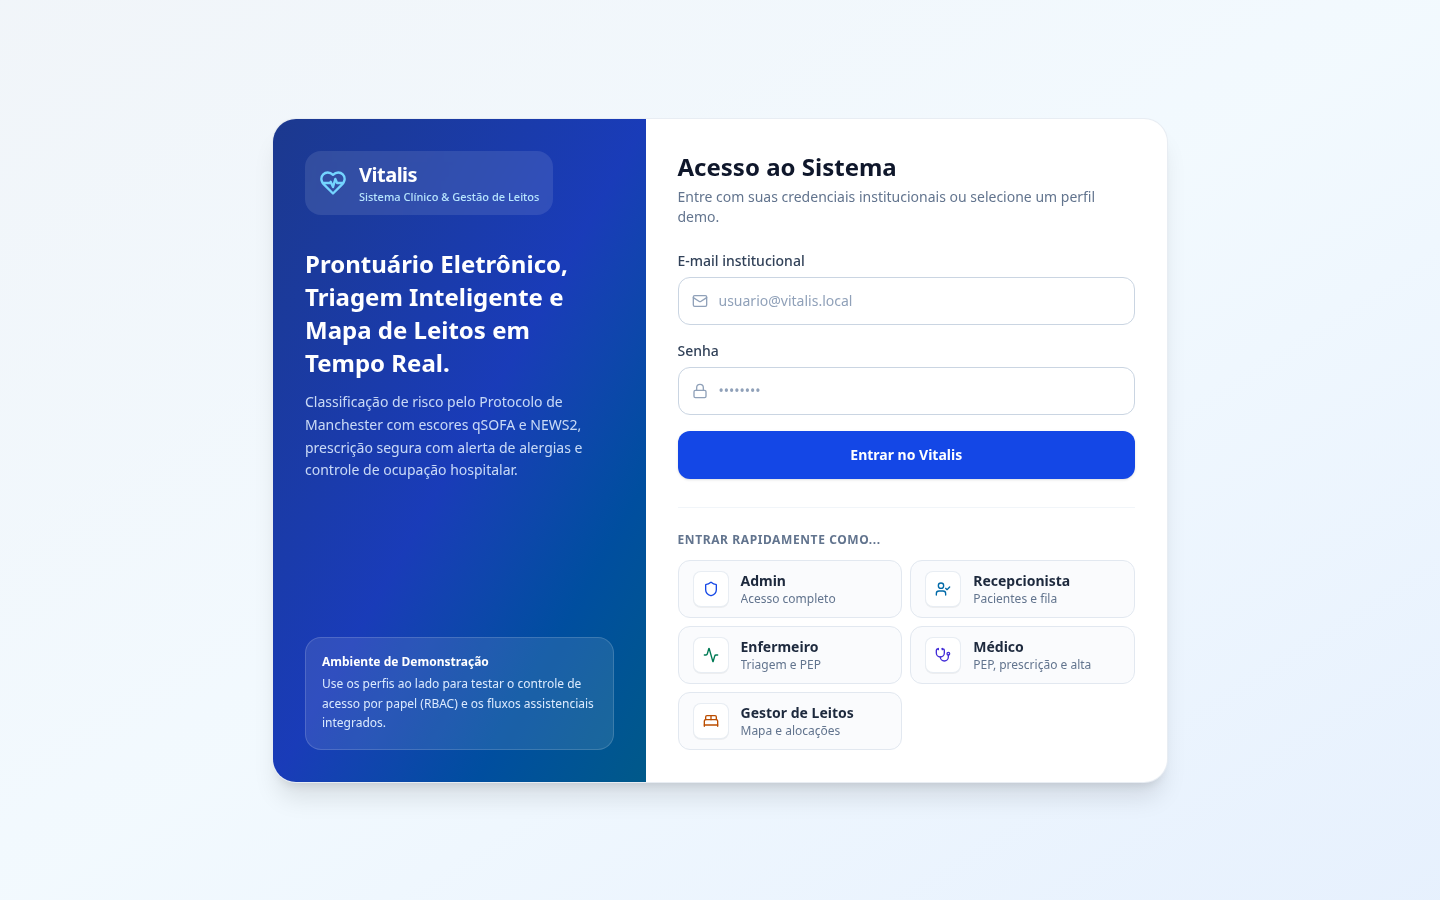
\includegraphics[width=0.92\textwidth]{imagens-telas/01-login.png}
    \caption{Tela de Login Institucional e Seleção Rápida de Perfis RBAC (\texttt{/login})}
    \label{fig:tela_01_login}
\end{figure}

% ==============================================================================
\subsection{Módulo de Recepção, Pacientes e Abertura de Atendimento}

O módulo de recepção (\texttt{/pacientes}) centraliza a busca instantânea por nome, CPF ou CNS (Figura~\ref{fig:tela_02_pacientes}), o cadastro com validação algorítmica de dígitos verificadores do CPF e geração automática do PEP (Figura~\ref{fig:tela_03_novo_paciente}), a gestão de contatos de emergência (Figura~\ref{fig:tela_04_contatos}) e a abertura de episódios de atendimento (Figura~\ref{fig:tela_05_abrir_atendimento}).

\begin{figure}[H]
    \centering
    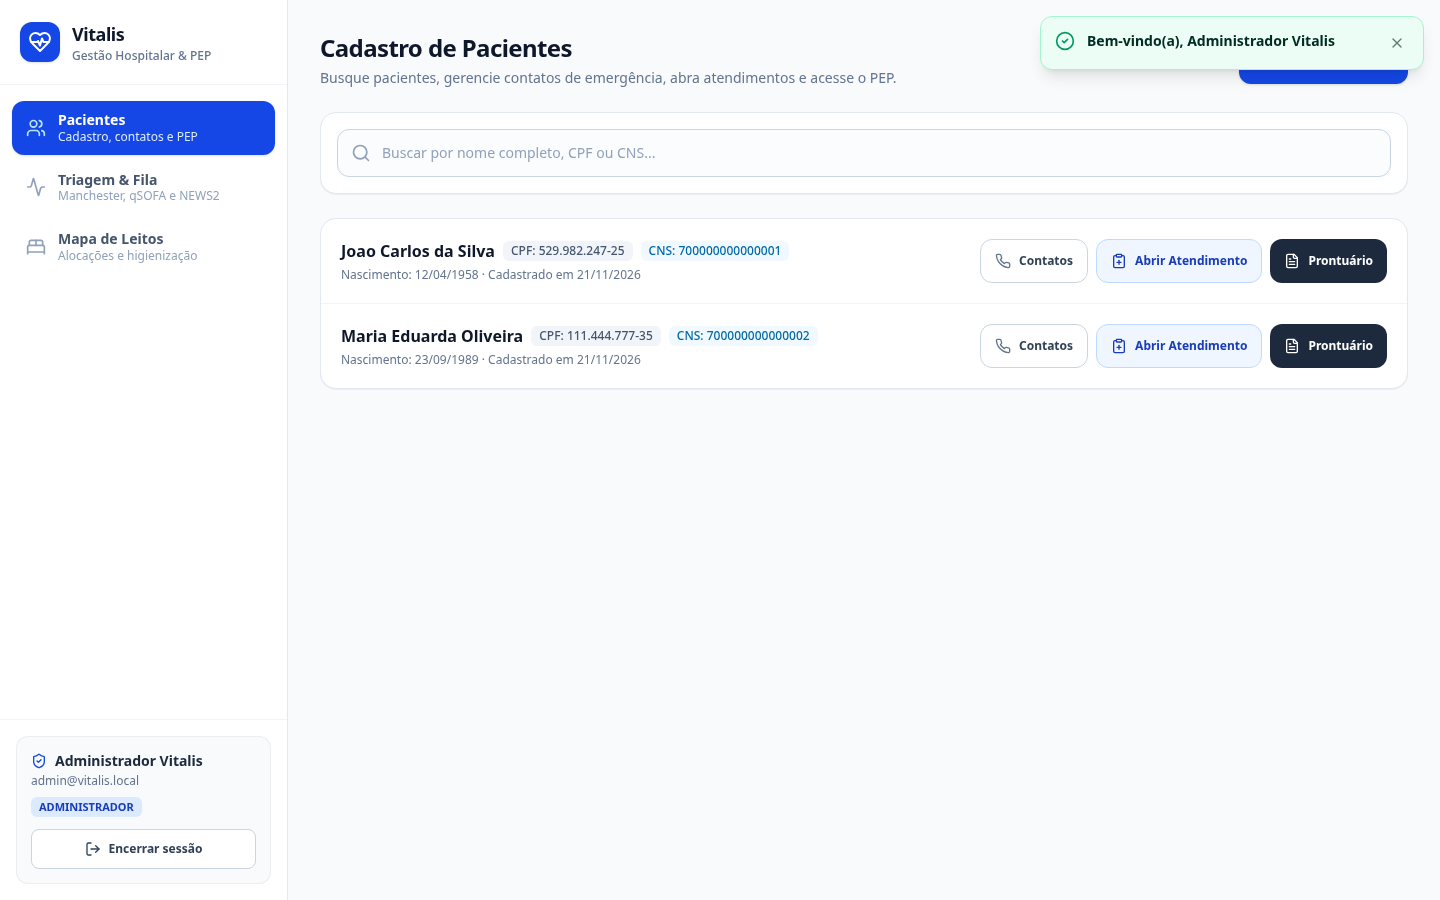
\includegraphics[width=0.92\textwidth]{imagens-telas/02-pacientes-lista.png}
    \caption{Listagem e Busca de Pacientes com Ações de Contatos, Atendimento e Prontuário}
    \label{fig:tela_02_pacientes}
\end{figure}

\begin{figure}[H]
    \centering
    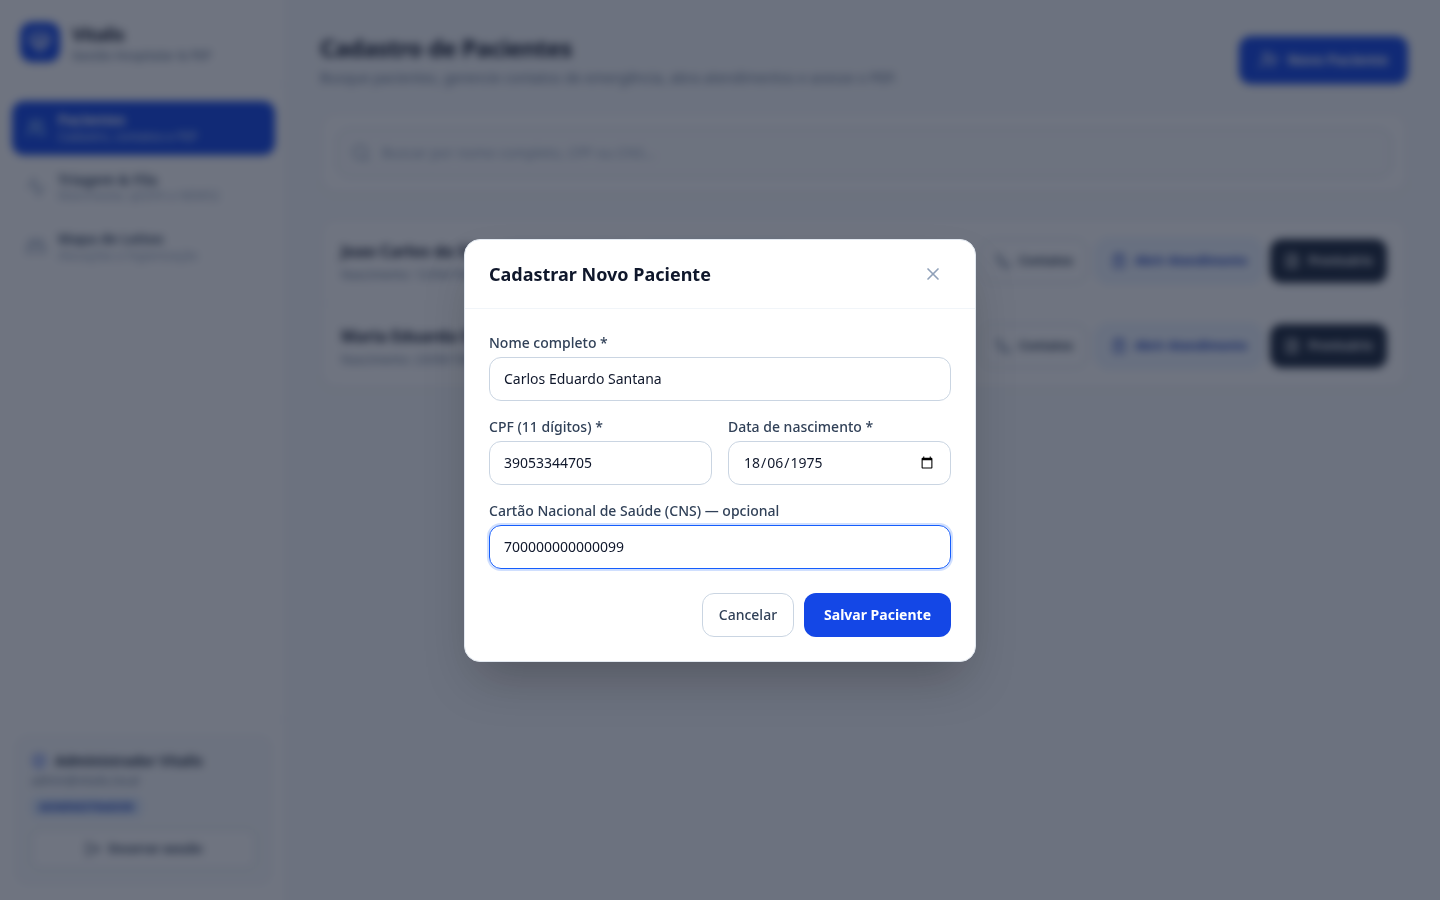
\includegraphics[width=0.88\textwidth]{imagens-telas/03-pacientes-novo-modal.png}
    \caption{Modal de Cadastro Unificado de Paciente com Validação de CPF e CNS (RF-002)}
    \label{fig:tela_03_novo_paciente}
\end{figure}

\begin{figure}[H]
    \centering
    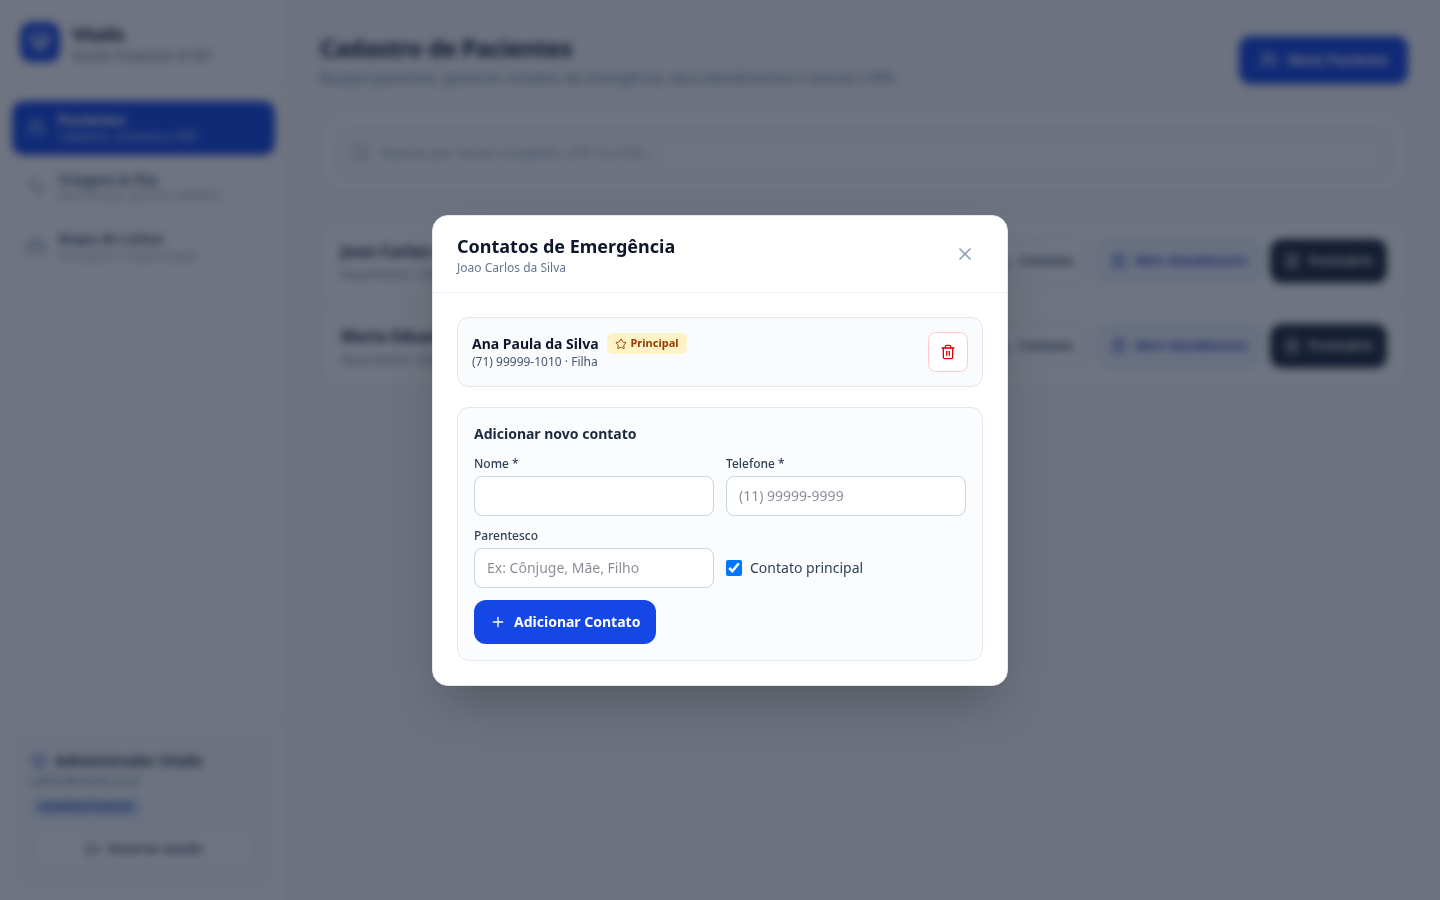
\includegraphics[width=0.88\textwidth]{imagens-telas/04-pacientes-contatos-emergencia.png}
    \caption{Gestão de Contatos de Emergência Vinculados ao Paciente (RF-002)}
    \label{fig:tela_04_contatos}
\end{figure}

\begin{figure}[H]
    \centering
    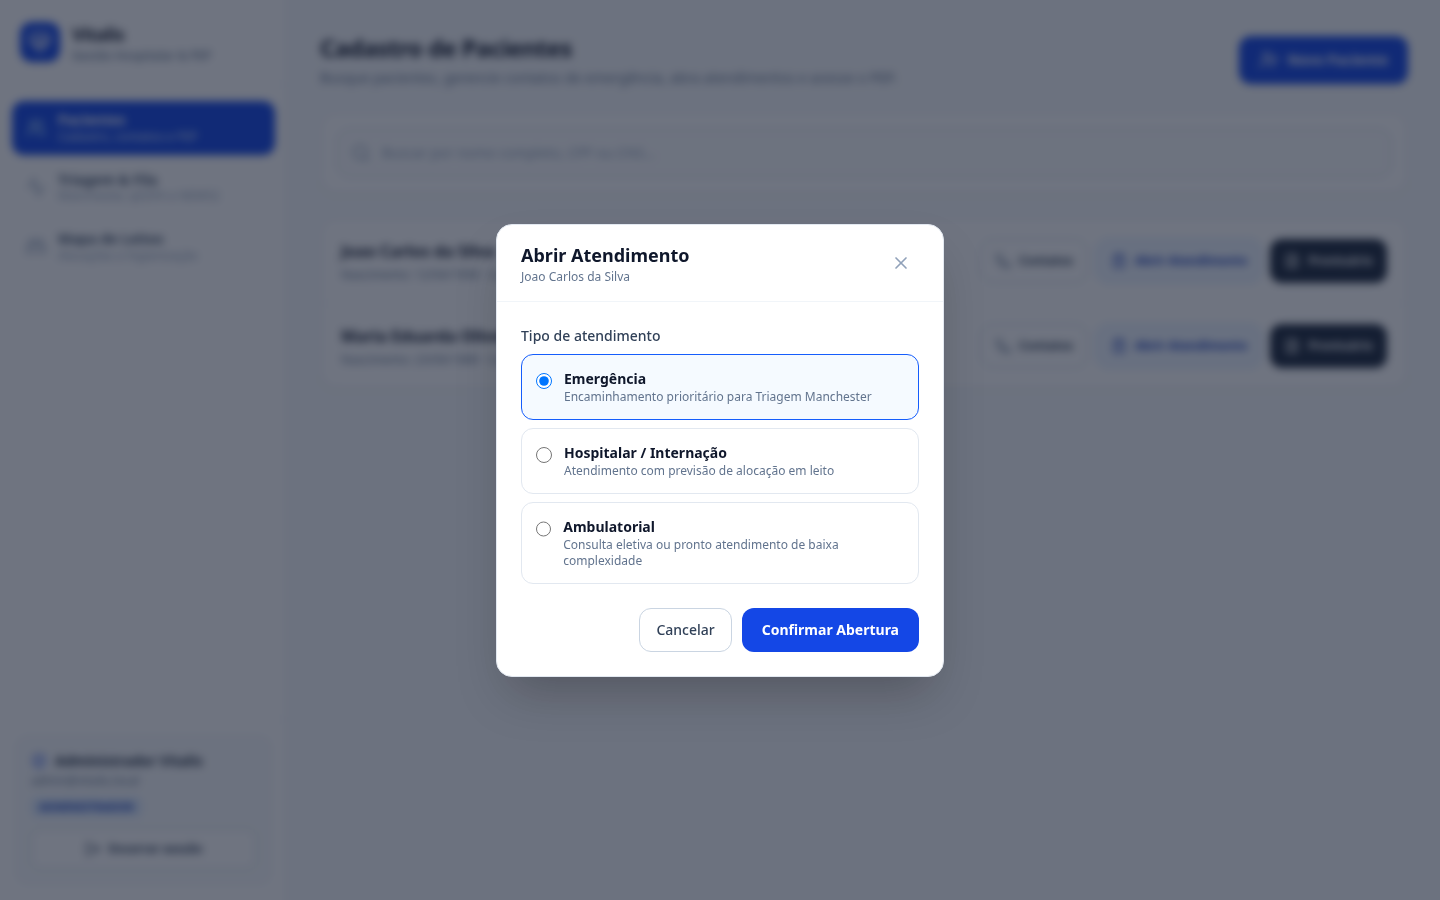
\includegraphics[width=0.88\textwidth]{imagens-telas/05-pacientes-abrir-atendimento.png}
    \caption{Modal de Abertura de Atendimento nas Modalidades Emergência, Hospitalar e Ambulatorial}
    \label{fig:tela_05_abrir_atendimento}
\end{figure}

% ==============================================================================
\subsection{Triagem de Manchester, Escores qSOFA/NEWS2 e Fila Prioritária}

Durante o preenchimento dos sinais vitais na estação de triagem (Figura~\ref{fig:tela_06_triagem_form}), o sistema calcula em tempo real a cor de prioridade do Protocolo de Manchester, os escores \textbf{qSOFA} e \textbf{NEWS2} e o alerta precoce de sepse (\textbf{RF-003 / RF-004}). Ao confirmar uma classificação \textbf{Vermelha (Emergência)}, o paciente é movido instantaneamente para o topo da fila, acionando o banner vermelho de emergência imediata e o alerta sonoro (Figura~\ref{fig:tela_07_fila_vermelha} --- \textbf{RN-001 / RF-021}).

\begin{figure}[H]
    \centering
    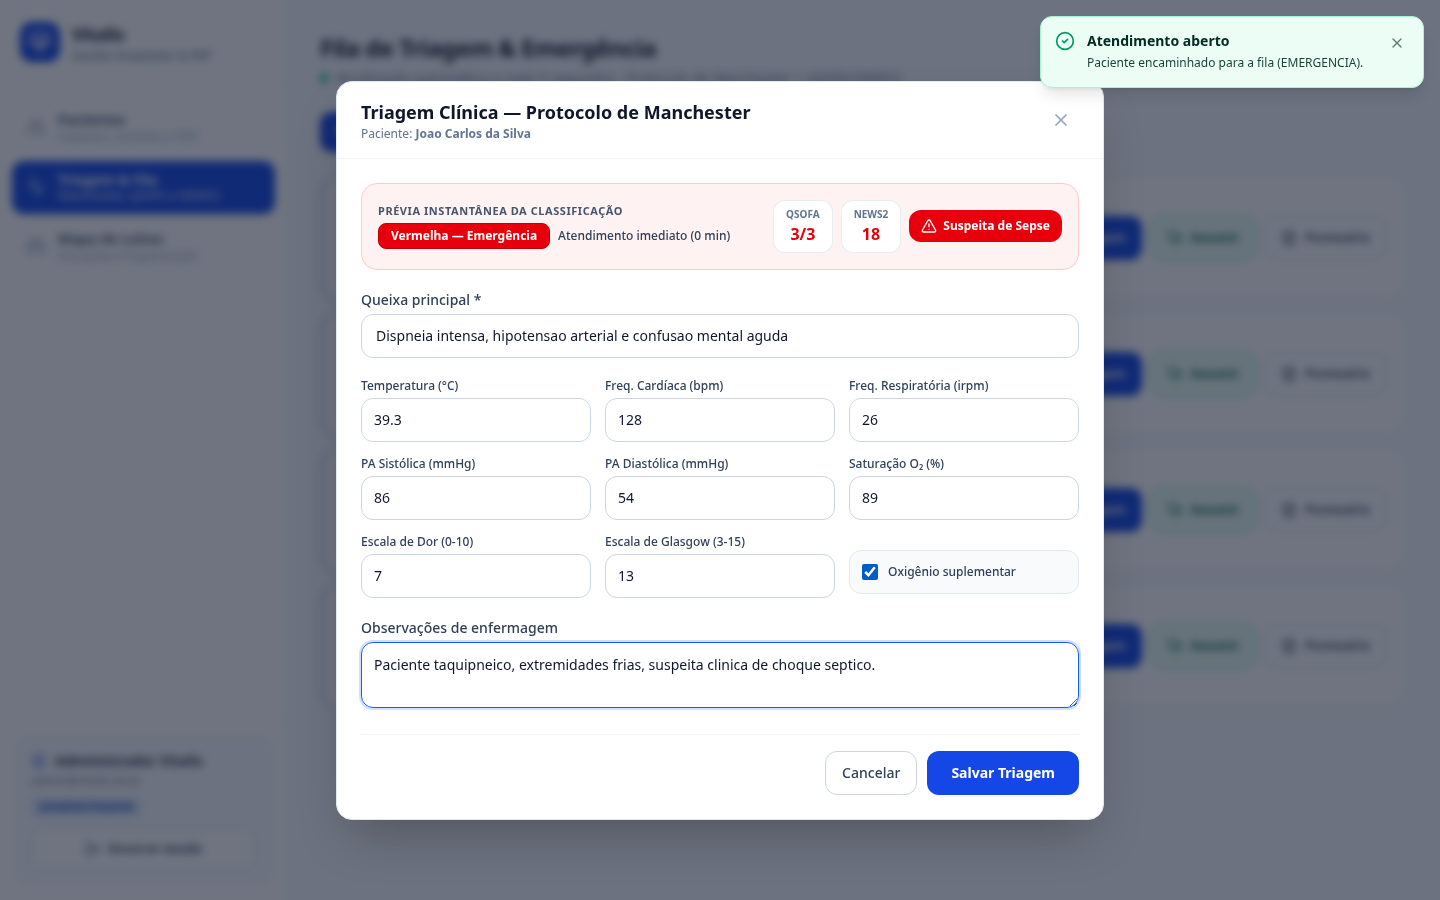
\includegraphics[width=0.92\textwidth]{imagens-telas/06-triagem-formulario-manchester-sepse.png}
    \caption{Formulário de Triagem com Prévia Instantânea de Manchester (Vermelha), qSOFA (3/3), NEWS2 e Suspeita de Sepse}
    \label{fig:tela_06_triagem_form}
\end{figure}

\begin{figure}[H]
    \centering
    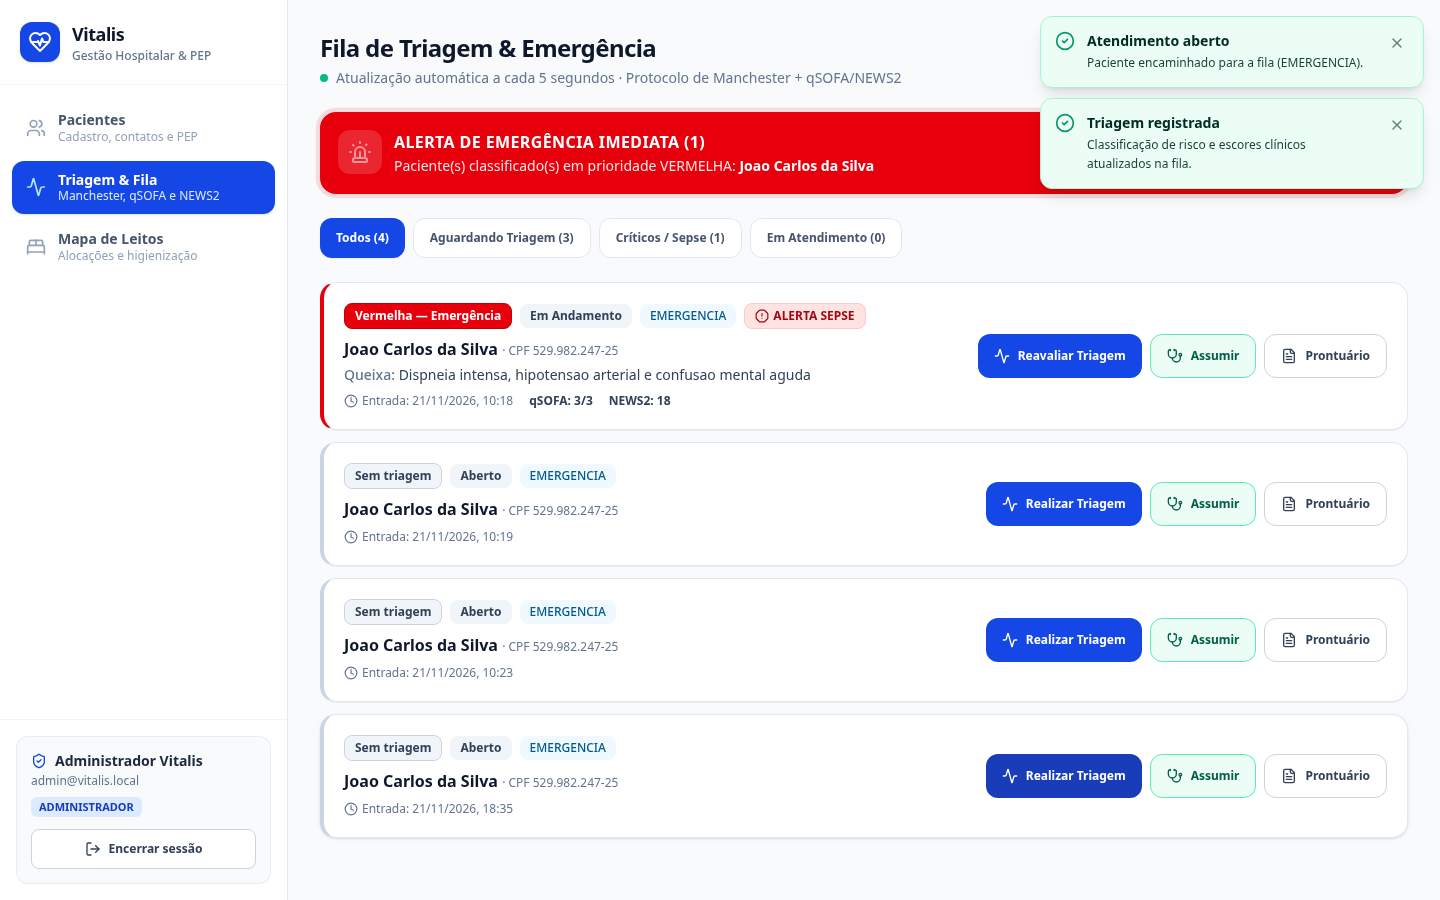
\includegraphics[width=0.92\textwidth]{imagens-telas/07-triagem-fila-alerta-vermelho.png}
    \caption{Fila Prioritária Reativa com Alerta de Emergência Imediata no Topo e Badge de Alerta Sepse (RN-001)}
    \label{fig:tela_07_fila_vermelha}
\end{figure}

% ==============================================================================
\subsection{Mapa Visual de Leitos, Alocação, Transferência e Higienização}

O painel de leitos (\texttt{/leitos}) apresenta a ocupação agrupada por ala em tempo real (Figura~\ref{fig:tela_08_mapa_leitos}), o fluxo de alocação condicionado à triagem prévia obrigatória (Figura~\ref{fig:tela_09_alocacao} --- \textbf{RN-004}), a transferência interna atômica que envia o leito de origem para higienização (Figura~\ref{fig:tela_10_transferencia} --- \textbf{RF-019}) e a trilha histórica de transições de status (Figura~\ref{fig:tela_11_historico} --- \textbf{RN-010}).

\begin{figure}[H]
    \centering
    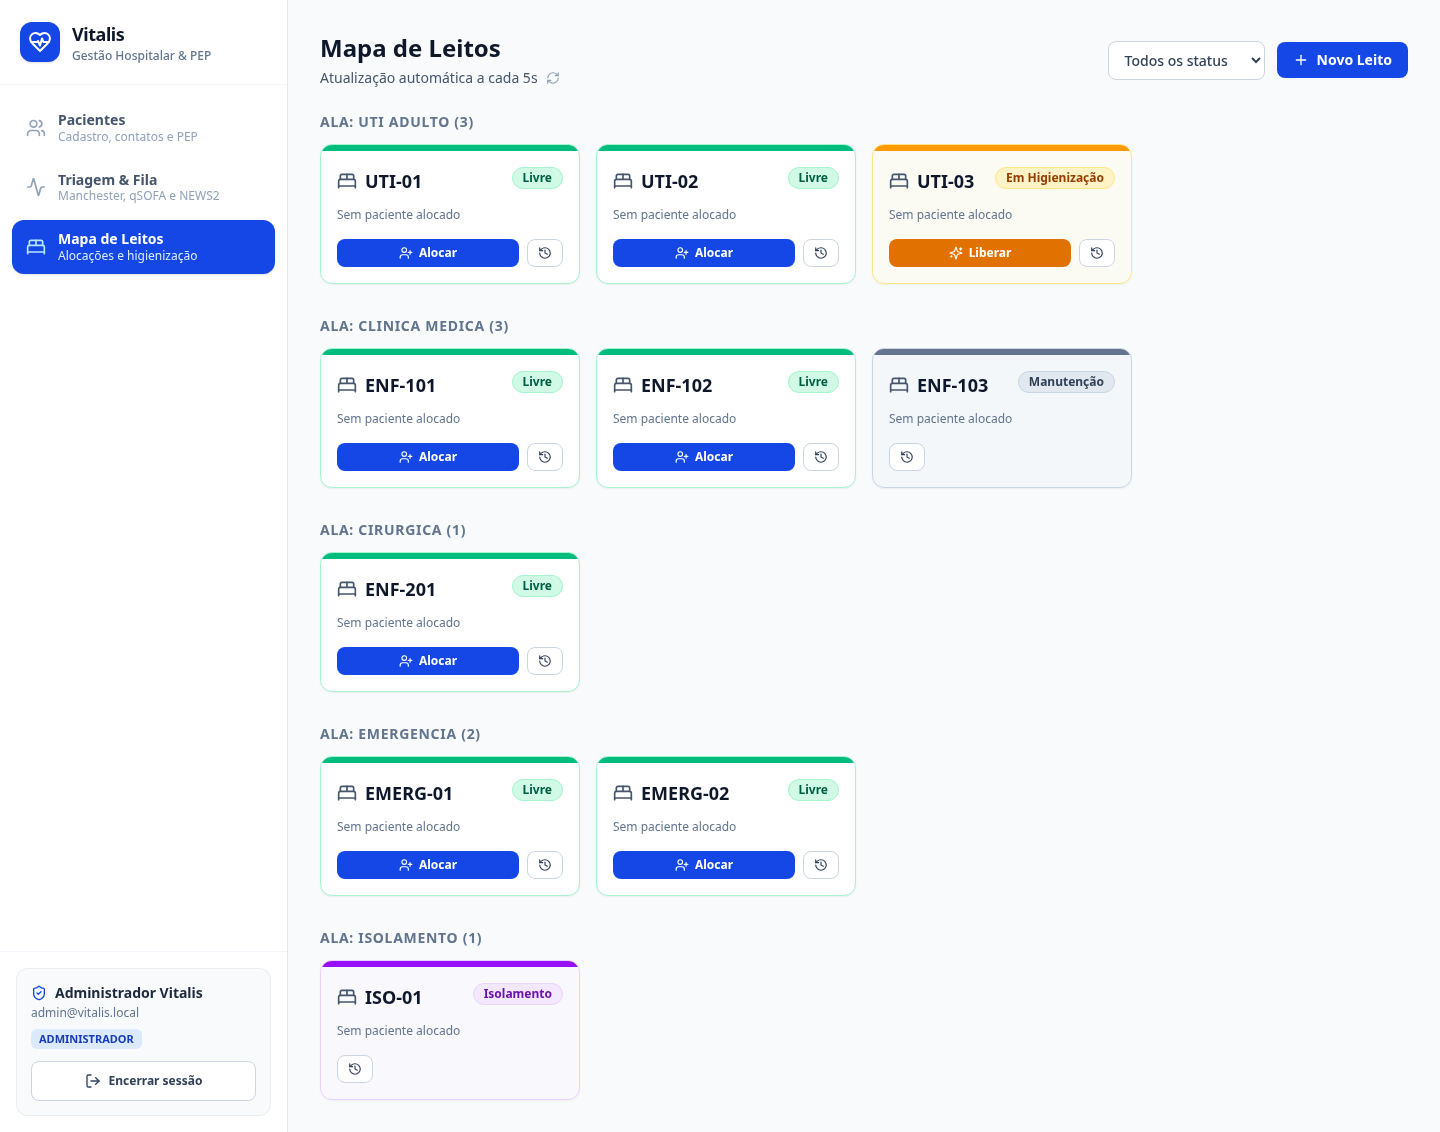
\includegraphics[width=0.92\textwidth]{imagens-telas/08-leitos-mapa-por-ala.png}
    \caption{Mapa Visual de Leitos Agrupado por Ala com Atualização Automática (RF-004)}
    \label{fig:tela_08_mapa_leitos}
\end{figure}

\begin{figure}[H]
    \centering
    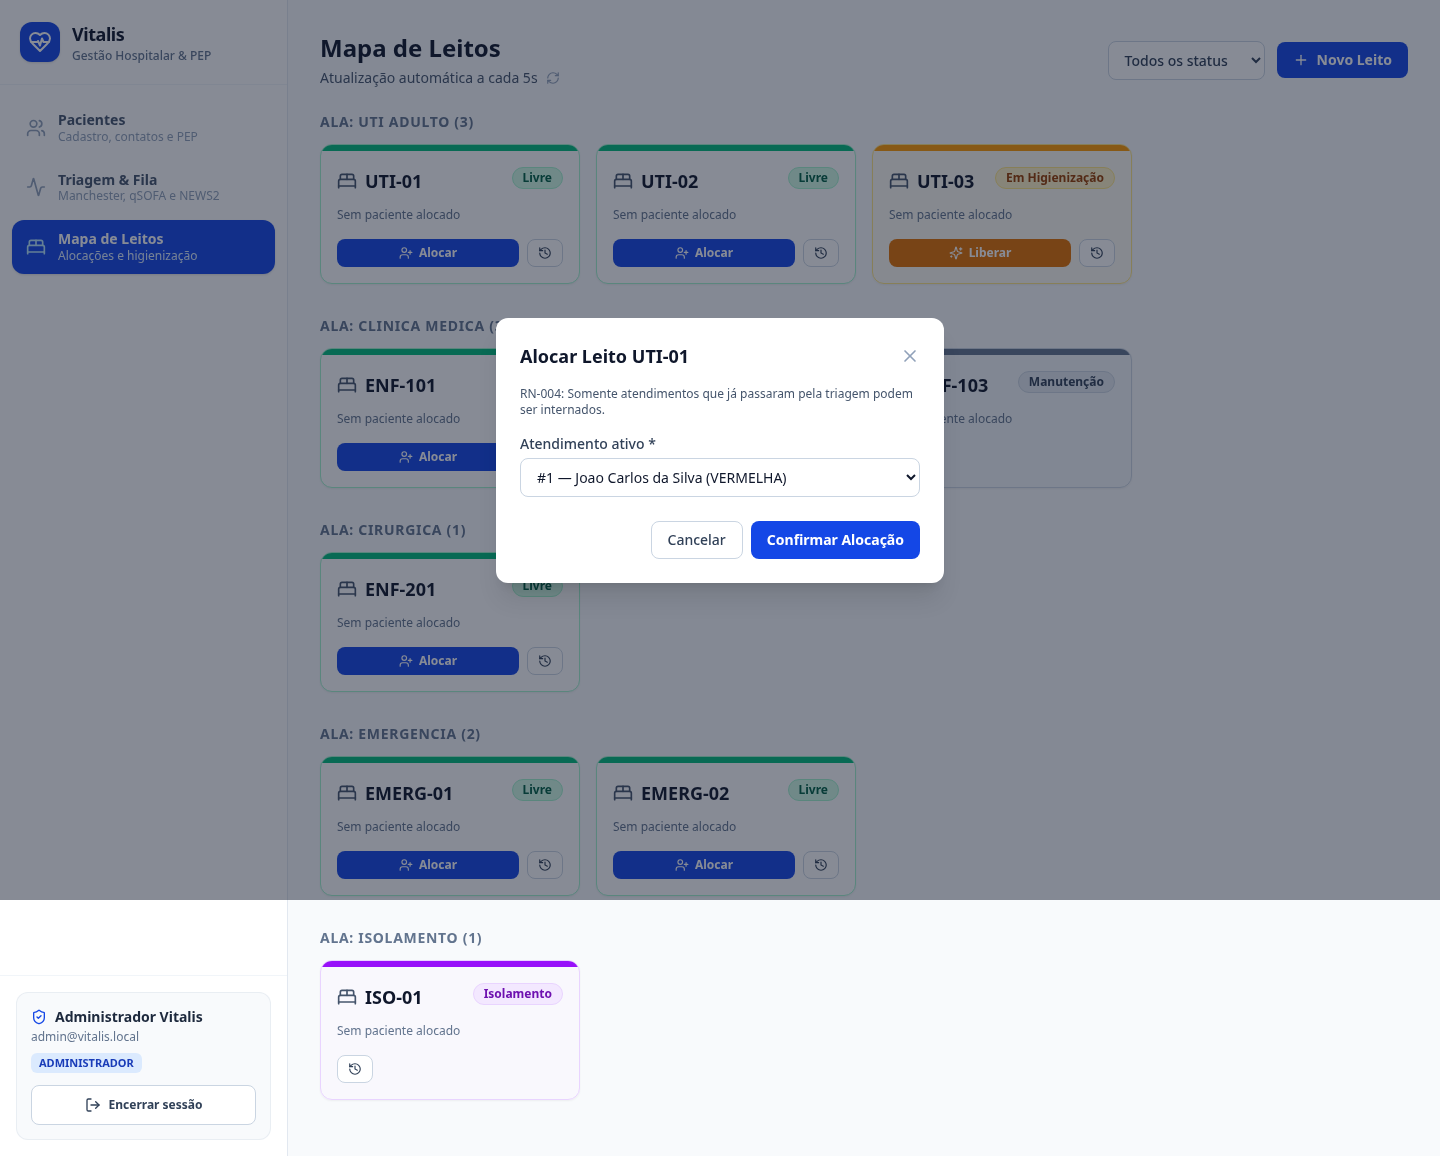
\includegraphics[width=0.88\textwidth]{imagens-telas/09-leitos-modal-alocacao.png}
    \caption{Modal de Alocação de Paciente em Leito com Validação Síncrona de Triagem Prévia (RN-004)}
    \label{fig:tela_09_alocacao}
\end{figure}

\begin{figure}[H]
    \centering
    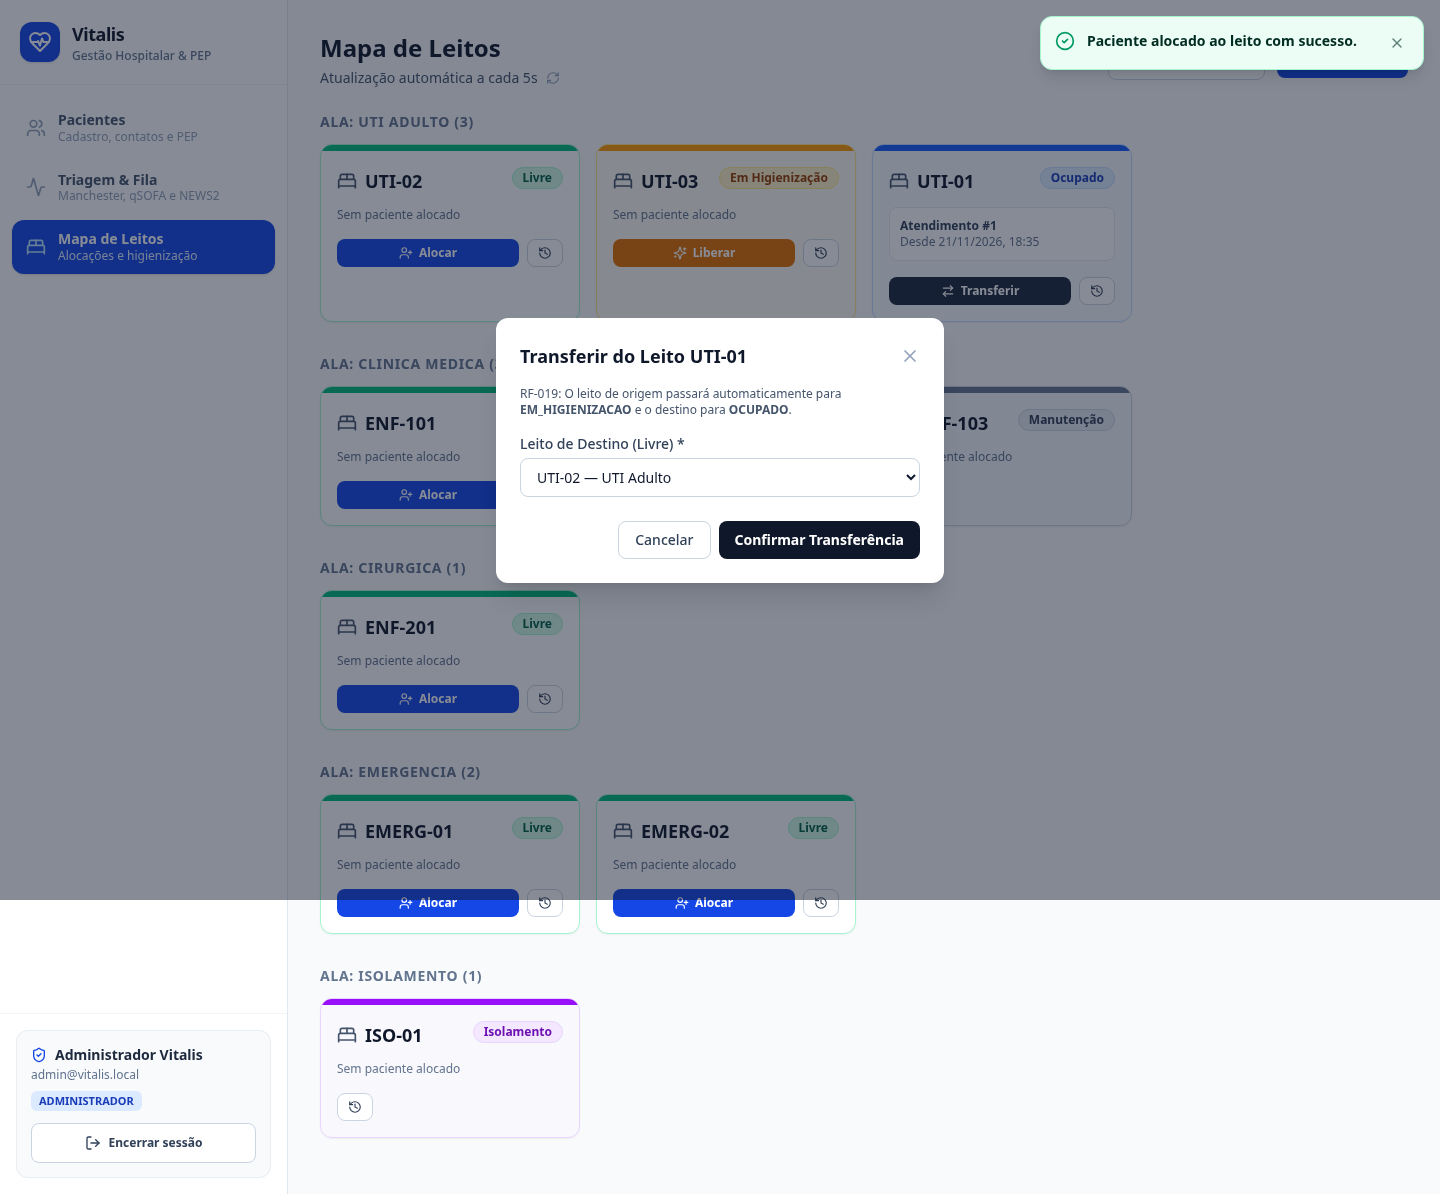
\includegraphics[width=0.88\textwidth]{imagens-telas/10-leitos-modal-transferencia.png}
    \caption{Modal de Transferência Interna entre Leitos e Alas (RF-019)}
    \label{fig:tela_10_transferencia}
\end{figure}

\begin{figure}[H]
    \centering
    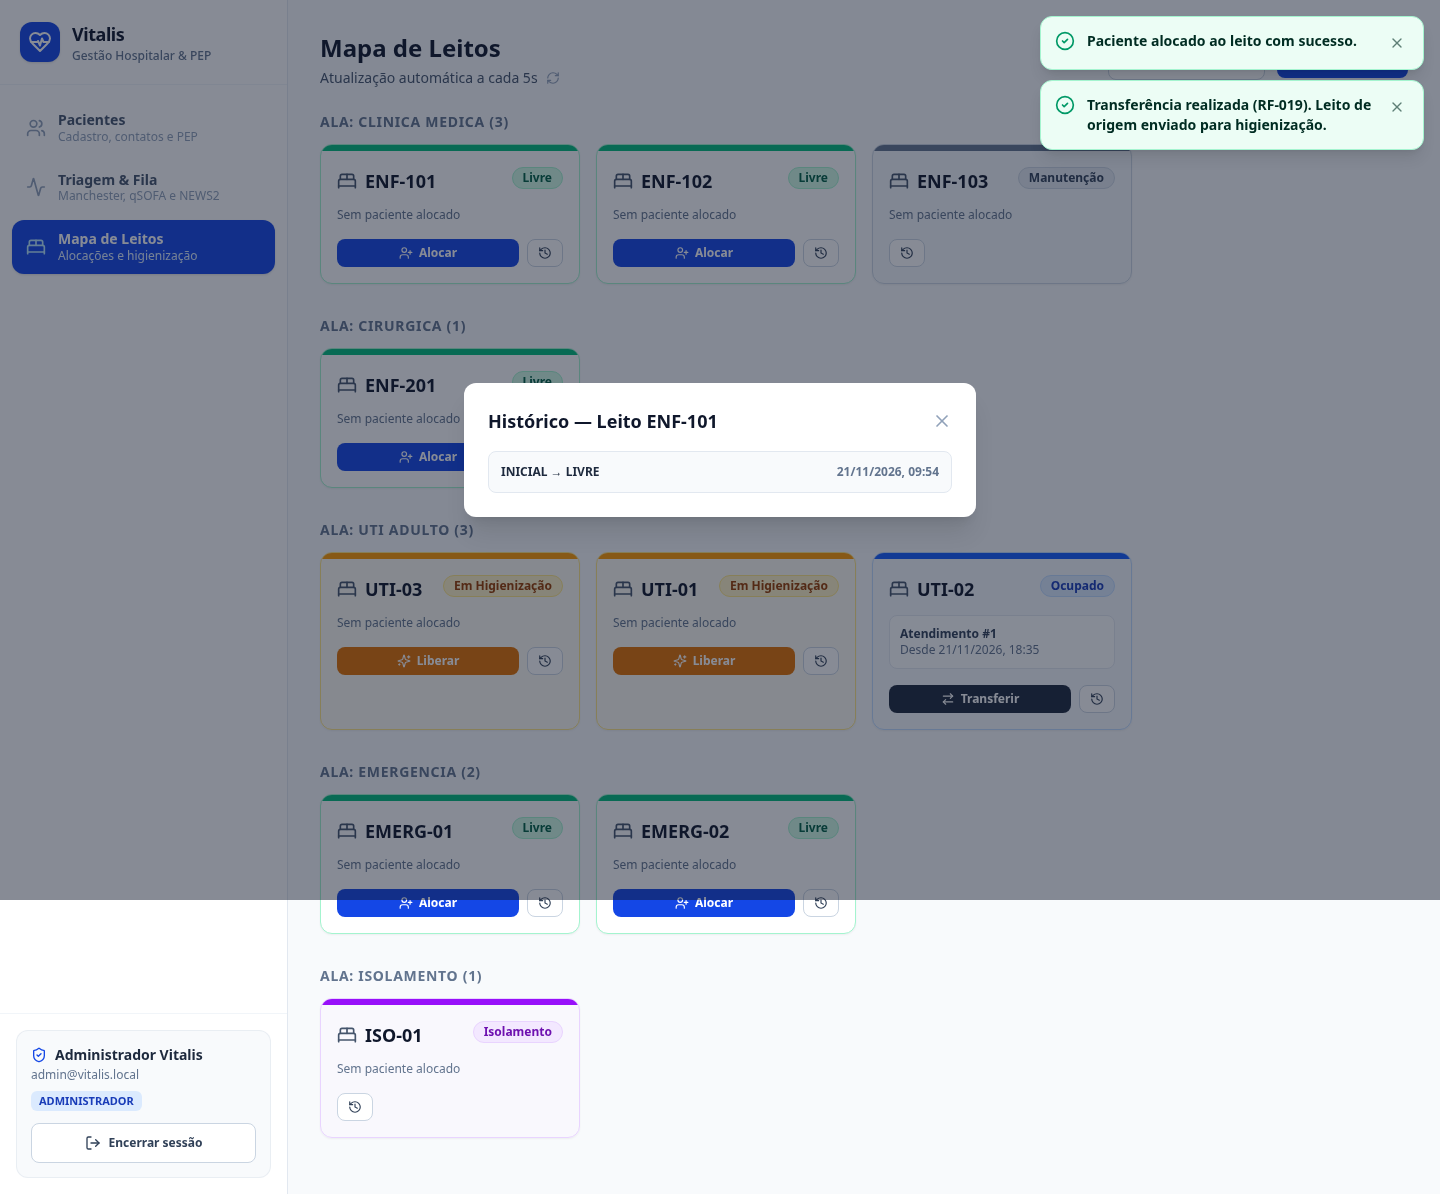
\includegraphics[width=0.88\textwidth]{imagens-telas/11-leitos-historico-higienizacao.png}
    \caption{Histórico Auditável de Alterações de Status e Higienização do Leito (RN-010)}
    \label{fig:tela_11_historico}
\end{figure}

% ==============================================================================
\subsection{Prontuário Eletrônico (PEP), Prescrição e Copiloto de IA com RAG}

O Prontuário Eletrônico do Paciente (\texttt{/pacientes/:id/prontuario}) exibe no topo a faixa vermelha de alergias ativas e consolida a linha do tempo clínica (Figura~\ref{fig:tela_12_pep_timeline}), o registro de evoluções de até 8.000 caracteres (Figura~\ref{fig:tela_13_evolucao}), a gestão de alergias (Figura~\ref{fig:tela_14_alergias}), o parecer consultivo do \textbf{Copiloto Farmacoterapêutico de IA com RAG e deliberação Human-in-the-Loop} (Figura~\ref{fig:tela_15_copiloto_ia} --- \textbf{RF-008 / RN-2}) e o modal obrigatório de reconhecimento de alergias antes da confirmação da prescrição (Figura~\ref{fig:tela_16_modal_rn008} --- \textbf{RN-008}).

\begin{figure}[H]
    \centering
    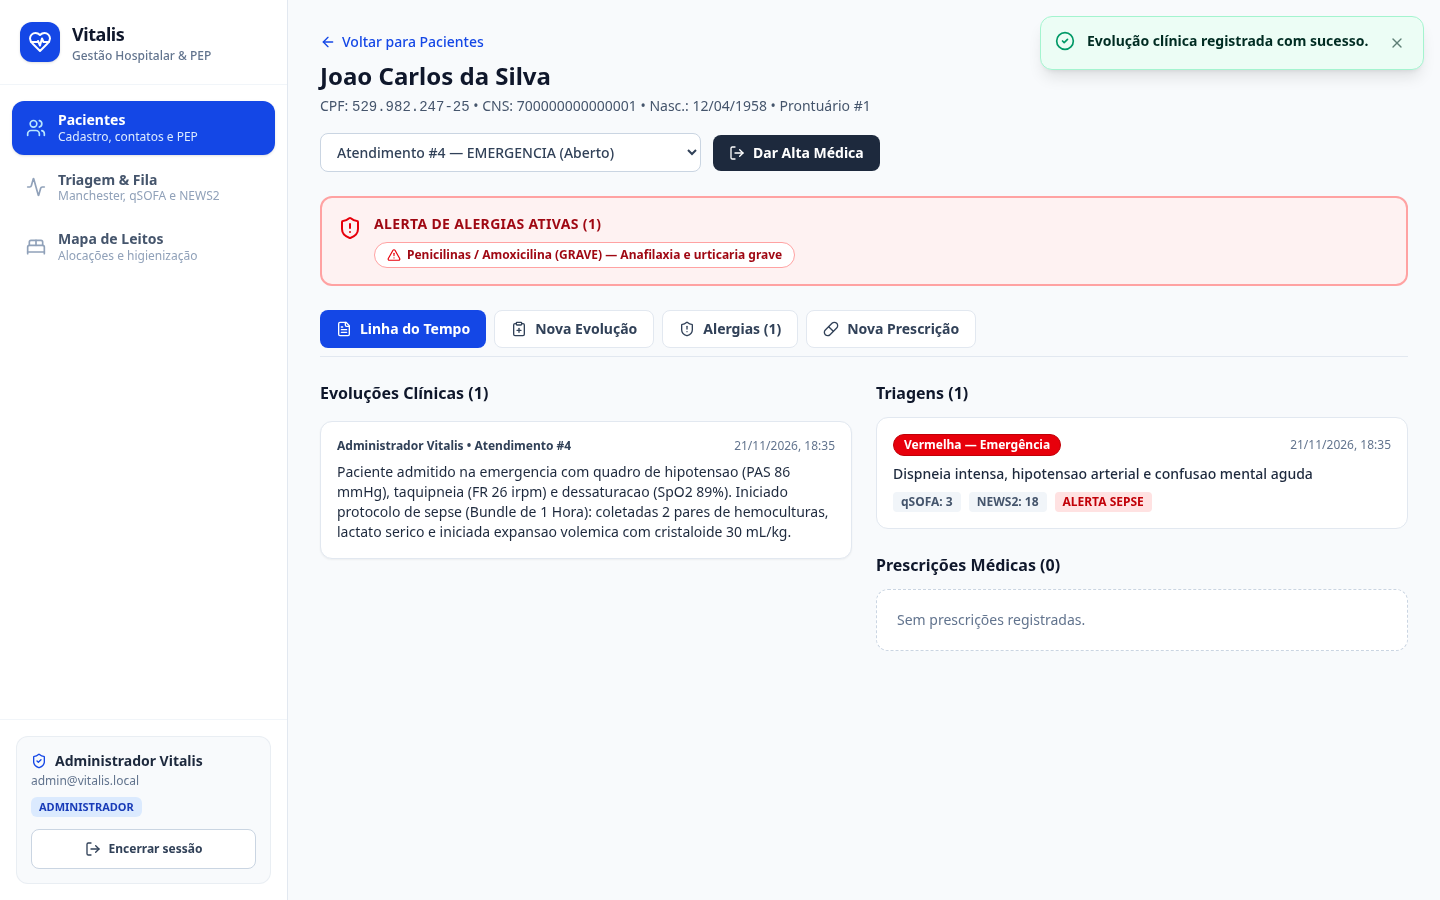
\includegraphics[width=0.92\textwidth]{imagens-telas/12-prontuario-linha-do-tempo.png}
    \caption{Prontuário Eletrônico (PEP) com Faixa de Alergias Graves e Linha do Tempo Consolidada (RF-005 / RF-018)}
    \label{fig:tela_12_pep_timeline}
\end{figure}

\begin{figure}[H]
    \centering
    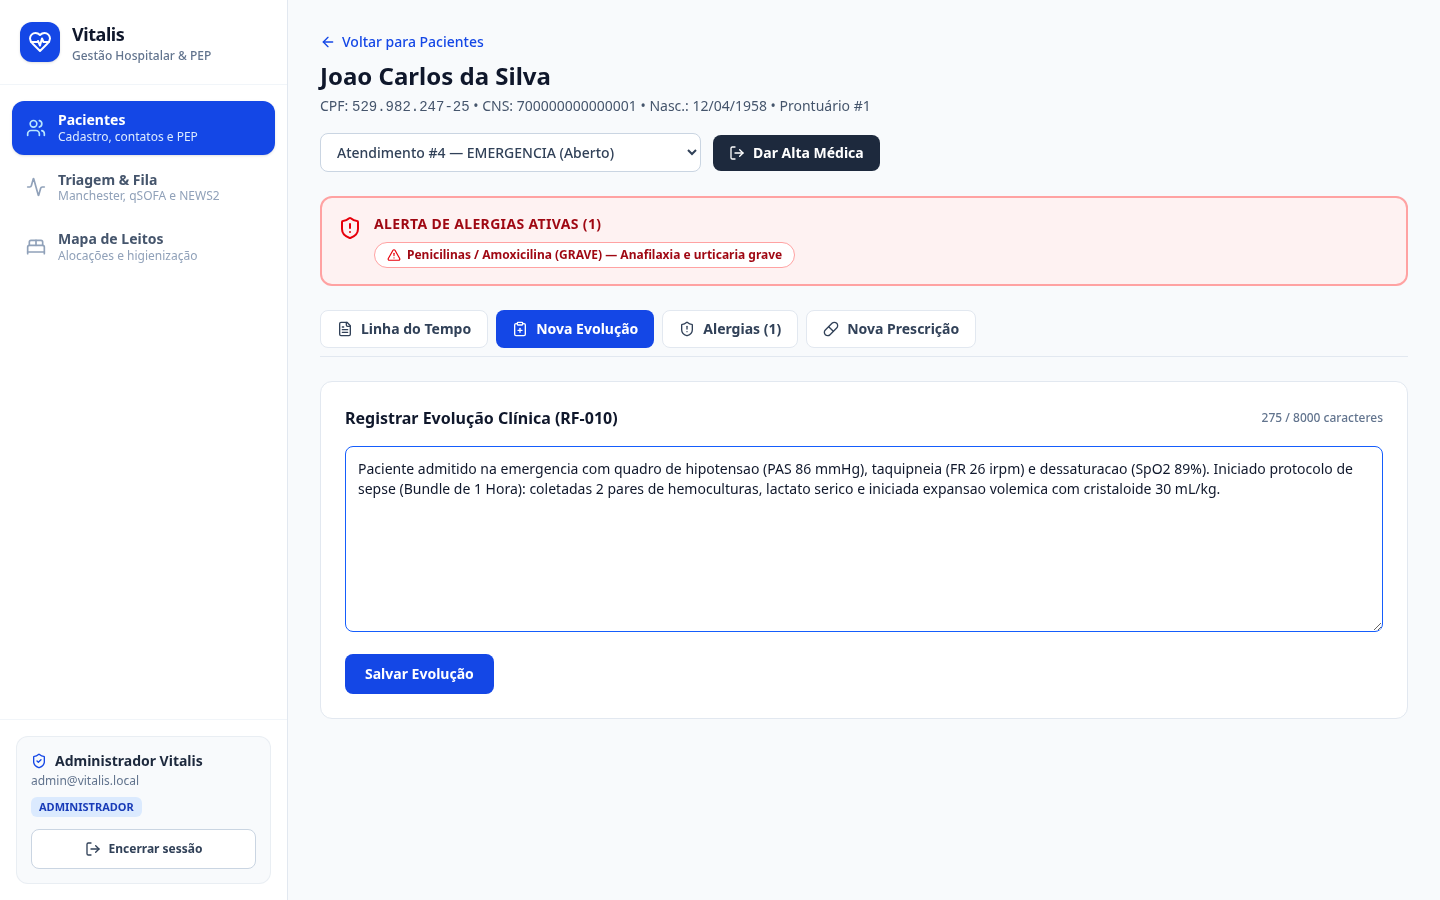
\includegraphics[width=0.92\textwidth]{imagens-telas/13-prontuario-nova-evolucao.png}
    \caption{Editor de Evolução Clínica com Contador para até 8.000 Caracteres (RF-010)}
    \label{fig:tela_13_evolucao}
\end{figure}

\begin{figure}[H]
    \centering
    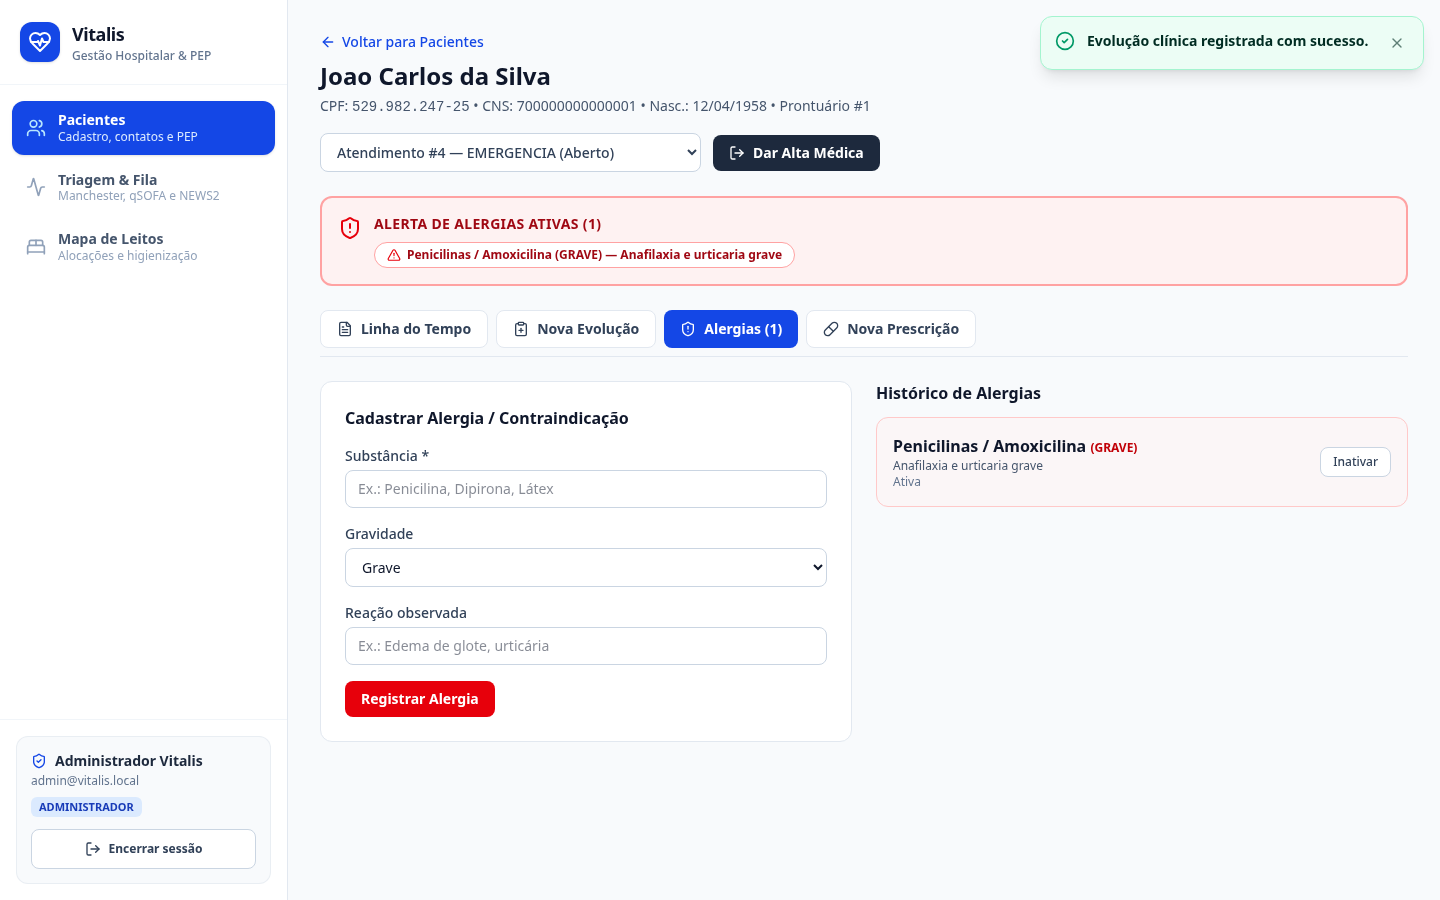
\includegraphics[width=0.92\textwidth]{imagens-telas/14-prontuario-alergias.png}
    \caption{Aba de Cadastro e Histórico de Alergias e Contraindicações no PEP (RF-018)}
    \label{fig:tela_14_alergias}
\end{figure}

\begin{figure}[H]
    \centering
    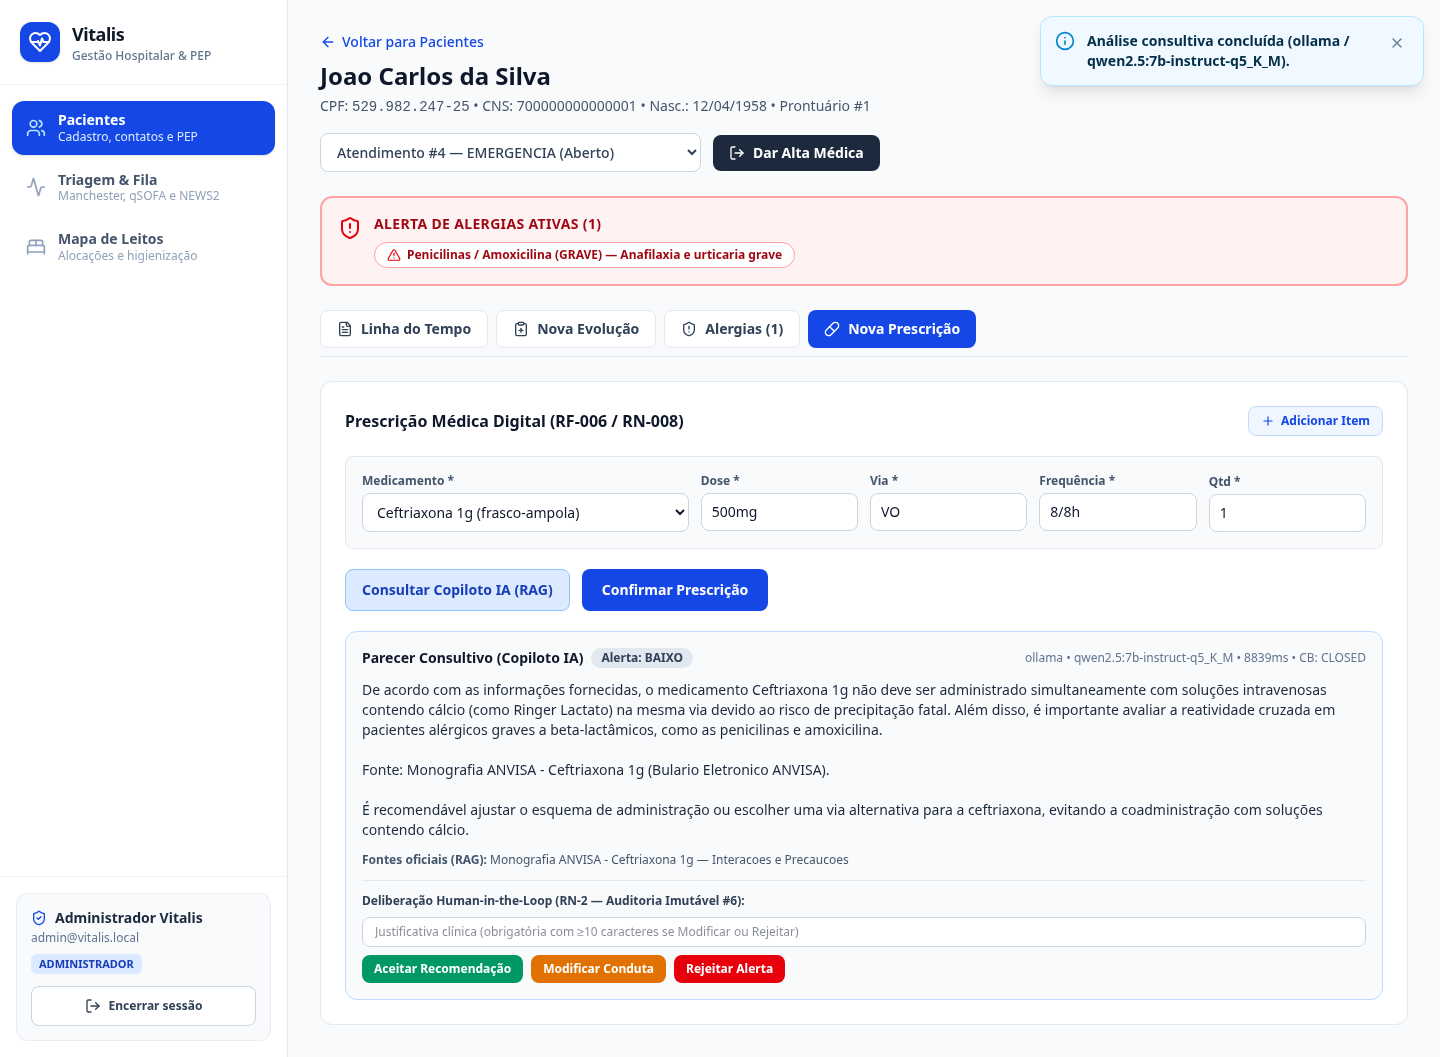
\includegraphics[width=0.95\textwidth]{imagens-telas/15-prontuario-prescricao-copiloto-ia.png}
    \caption{Prescrição Médica Assistida pelo Copiloto de IA (\texttt{ollama / qwen2.5:7b-instruct-q5\_K\_M}) com Citação da Monografia ANVISA e Deliberação Human-in-the-Loop (RF-008 / RN-2)}
    \label{fig:tela_15_copiloto_ia}
\end{figure}

\begin{figure}[H]
    \centering
    
\includegraphics[width=0.90\textwidth]{imagens-telas/16-prontuario-modal-alergia-rn008.png}
    \caption{Modal Obrigatório de Reconhecimento Explícito de Alergias na Prescrição (RN-008)}
    \label{fig:tela_16_modal_rn008}
\end{figure}

% ==============================================================================
\subsection{Alta Hospitalar Assistida por IA e Imutabilidade Pós-Alta}

No encerramento do atendimento, o médico pode gerar a minuta estruturada de sumário de alta via IA (Figura~\ref{fig:tela_17_alta_ia} --- \textbf{RF-011 / RF-012}). Uma vez homologada a alta, o leito é enviado automaticamente para \texttt{EM\_HIGIENIZACAO} e o prontuário daquele episódio é permanentemente trancado contra edições retroativas (Figura~\ref{fig:tela_18_pep_trancado} --- \textbf{RN-12}).

\begin{figure}[H]
    \centering
    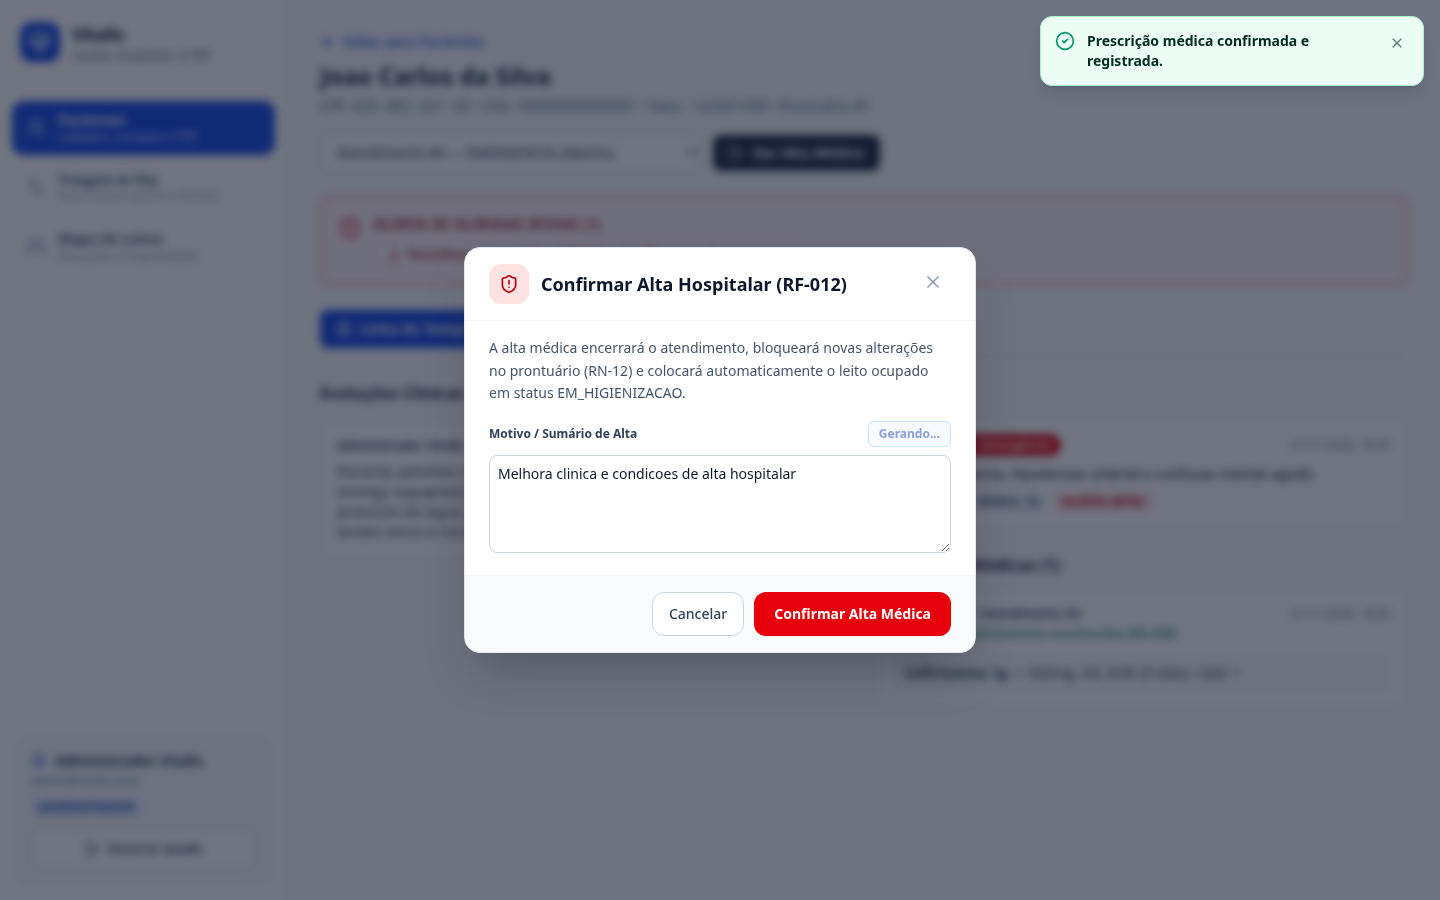
\includegraphics[width=0.90\textwidth]{imagens-telas/17-prontuario-modal-alta-minuta-ia.png}
    \caption{Modal de Alta Hospitalar com Geração de Minuta de Sumário de Alta por IA (RF-011 / RF-012)}
    \label{fig:tela_17_alta_ia}
\end{figure}

\begin{figure}[H]
    \centering
    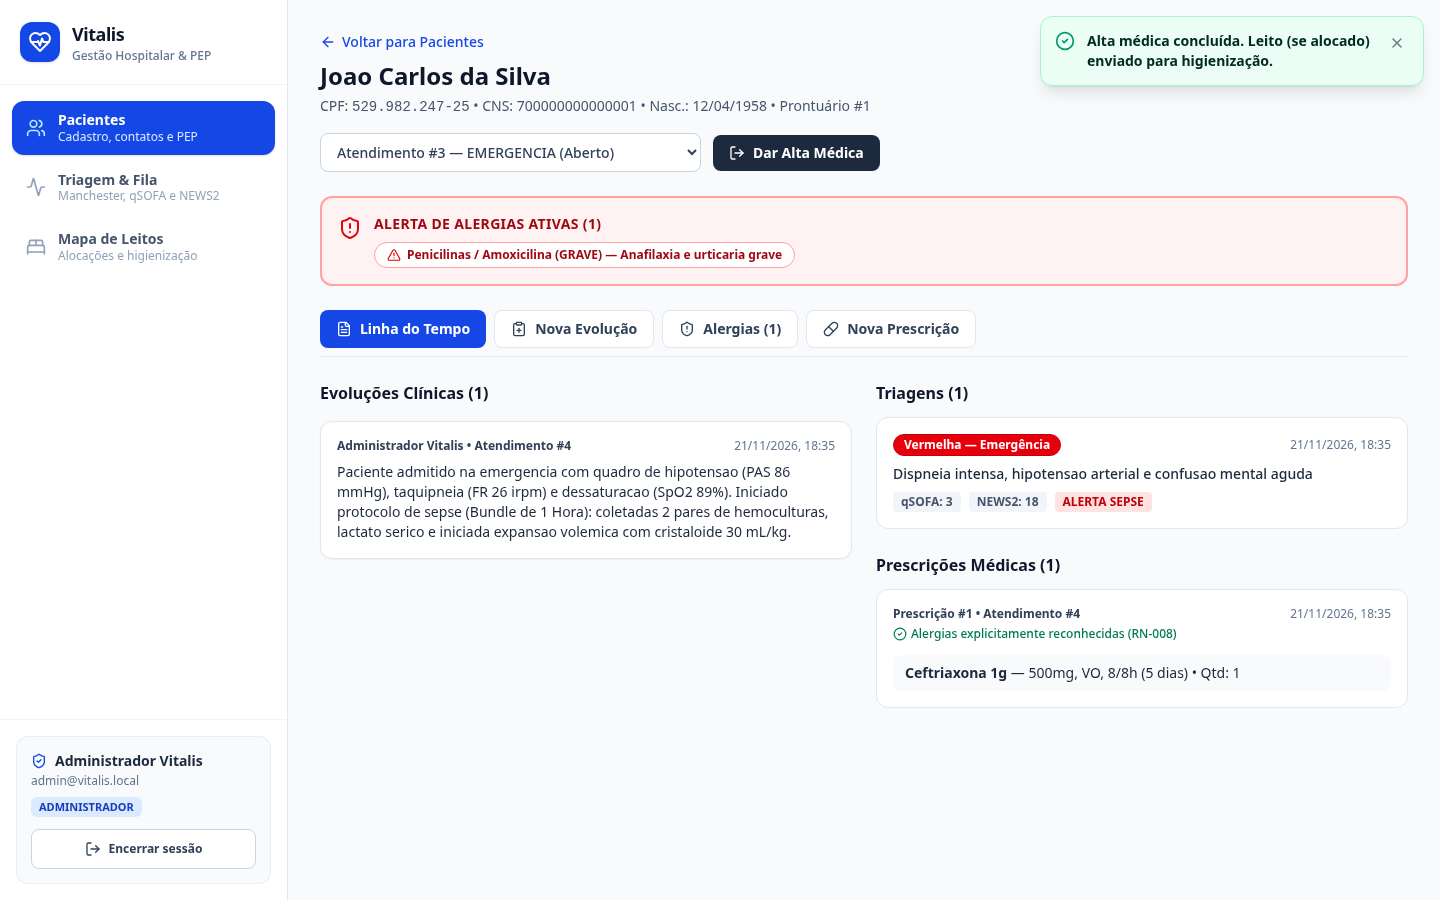
\includegraphics[width=0.92\textwidth]{imagens-telas/18-prontuario-encerrado-rn12.png}
    \caption{Prontuário Encerrado após a Alta Médica com Bloqueio de Escrituração Retroativa (RN-12)}
    \label{fig:tela_18_pep_trancado}
\end{figure}
